% !TEX root = ./repair.tex

\section{Simulation studies}
\label{sec:experiments}
%\let\beta\theta

\subsection{Over-parameterized linear models}


We begin by giving further details of the simulation briefly discussed
in Section~\ref{sec:overview}. In this experiment we simulate underdetermined linear models where $p > n$.
We generate $n$ data points $(X_i, y_i)$ where
$y_i = X_i^T \theta^* + w_i$ with $w_i$ an additive noise term. We then compute the minimum norm estimator
\begin{equation}
  \hat\theta = X^T (X X^T)^{-1} y
\end{equation}
The estimated model is corrupted to
\begin{equation}
  \eta = \hat\theta + z
\end{equation}
where $z_j \sim (1-\epsilon) \delta_0 +\epsilon Q$. The corrupted estimator is then repaired by performing median regression:
\begin{align}
  \tilde u &= \argmin \|\eta - X^T u\|_1 \\
  \tilde \theta &= X^T \tilde u.
\end{align}
The \texttt{quantreg} package in $R$ is used to carry out the median regression (quantile regression for quantile level $\tau = \frac{1}{2}$) using the Frisch-Newton interior point algorithm to solve the linear program (method \texttt{fn} in this package).

The design is sampled as $X_{ij} \sim N(0,1)$ and we take $\theta_j^* \sim N(0,1)$ and $Q = N(1,1)$. In the plots shown
in Figure~\ref{fig:exp1} the sample size is fixed at $n=100$ and the dimension $p$ is varied according to $p/n=200/j^2$
for a range of values of $j$. The plots show the empirical probability of exact repair $\tilde\theta = \hat\theta$ as a function of $\epsilon$. Each point on the curves is the average repair success over $500$ random trials.
The roughly equal spacing of the curves agrees with the theory, which indicates that $\sqrt{n/p}/(1-\epsilon)$ should be sufficiently small for successful repair.

\begin{figure}[t]
  \begin{center}
    \begin{tabular}{cc}
      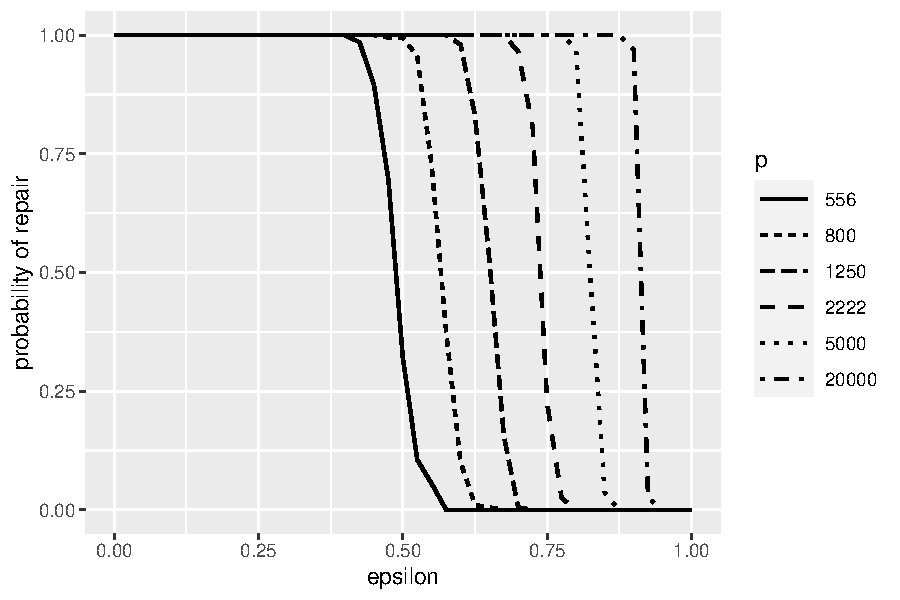
\includegraphics[width=.47\textwidth]{fig/plot-linear-100} &
      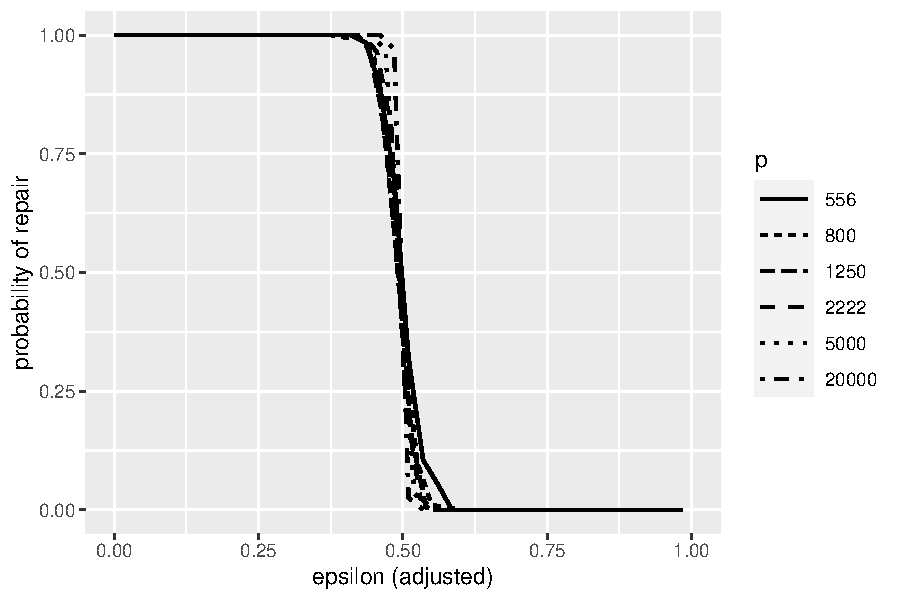
\includegraphics[width=.47\textwidth]{fig/plot-linear-100-adj}\\[-10pt]
    \end{tabular}
  \end{center}
\caption{Model repair for underdetermined linear models $y=X^T\theta + w$ with $p>n$. The left plot shows the empirical probability of successful model repair for $n=100$ with the model dimension $p$
varying as $p/n = 200 /j^2$, for $j=1,\ldots, 7$. Each point is an average over 500 random trials. The covariates are sampled as $N(0,1)$ and the corruption distribution is $Q=N(1,1)$. The right plot shows the repair probablity as a function
of the adjusted corruption probability $\tilde\epsilon_j = \epsilon + c'\cdot j - \frac{1}{2}$.}
\label{fig:exp1}
\end{figure}


\subsection{Random features models trained with gradient descent}

In this experiment we simulate over-parameterized random features models.
We generate $n$ data points $(X_i, y_i)$ where
$y_i = X_i^T \theta^* + w_i$ with $w_i$ an additive noise term. The covariates are generated
as a layer of a random neural network, with $X_i = \tanh(WZ_i)$ where $Z_i \in\reals^d$ with $Z_{ij} \sim N(0,1)$
and $W\in\reals^{p\times d}$ with $W_{ij} \sim N(0, 1/d)$. We then approximate the least squares
solution using gradient descent intialized at zero, with updates
\begin{equation}
  \hat\theta^{(t)} = \hat\theta^{(t-1)} + \frac{\eta}{n} X^T R^{(t-1)}
\end{equation}
where the residual vector $R^{(t-1)}\in\reals^n$ is given by $R_i = (y_i - X_i^ T\hat\theta^{(t-1)})$.
The step size $\eta$ is selected empirically to insure convergence in under $1{,}000$ iterations.
Figure~\ref{fig:rf} shows two sets of results, for $n=50$ and $n=100$. For each value of the final dimension $p$,
three values of the original data dimension $d$ are selected: $d=p$, $d=\lceil 2p/3\rceil$,
and $d=\lceil p/2\rceil$. The recovery success curves for gradient descent are similar to those obtained for the minimal norm solution.

\begin{figure}[t]
  \begin{center}
    \begin{tabular}{cc}
      {\scriptsize $n=50$} & {\scriptsize $n=100$} \\
      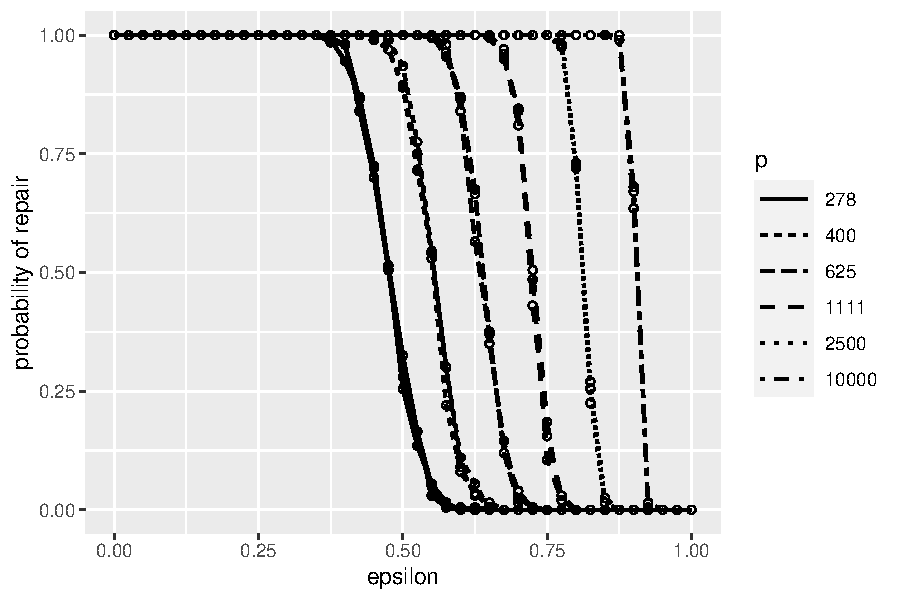
\includegraphics[width=.47\textwidth]{fig/plot-rf-50} &
      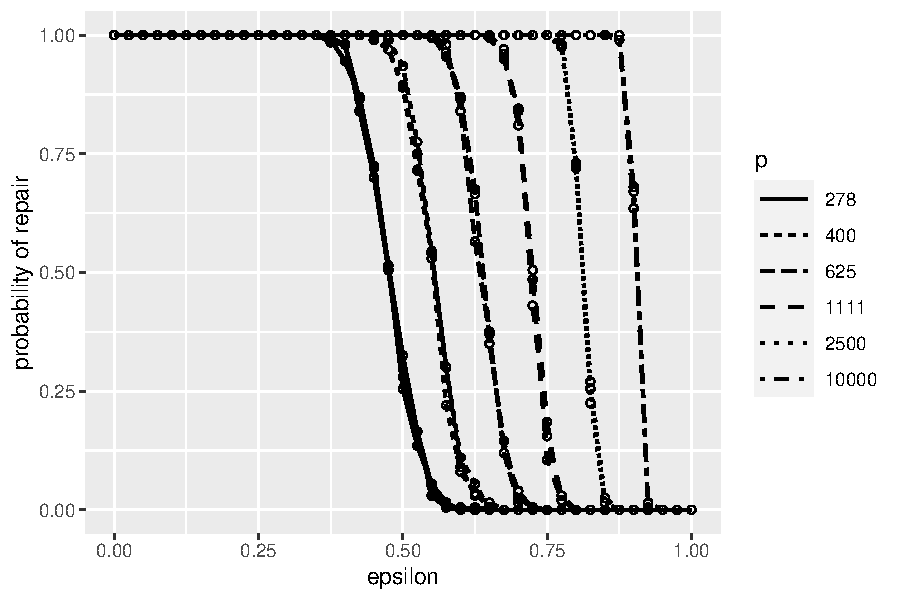
\includegraphics[width=.47\textwidth]{fig/plot-rf-100}\\[-10pt]
    \end{tabular}
  \end{center}
\caption{Model repair for random feature models $y=\psi(XW)\theta + w$ with $p>n$, where $\psi(\cdot) = \tanh(\cdot)$
for $n=50$ (left) and $n=100$ (right). For each value of $p$, three values of $d$ are evaluated, $d=p$, $d=\lceil 2p/3\rceil$,
and $d=\lceil p/2\rceil$; the results are effectively the same for each $d$.}
\label{fig:rf}
\end{figure}
